% -*- TeX-master: "all_the_notes.tex" -*-

\newpage
\section{Resonators}\label{sec:transmission-line}

\subsection{Deriving resonator equations}
\label{sec:deriv-reson-equat}


We treat the transmission line as  a chain of inductors and capacitors
and that is lossless (i.e $ R=0 $ and $ G=0 $ = no conductance between
the lines) with

  \begin{equation}
    l \approx \mu_0 \text{ - the inductance per unit length}\qquad c \approx \epsilon_0 \text{ - the capacitance per unit length},
  \end{equation}

  \noindent  as  shown in  Fig.\ref{transtLine}.   Recall  that for  a
  device    of   size    $   \alpha    $,   the    capacitance   will    be
  $ C \approx  \epsilon_0\alpha $.  The current and the  voltage in the line
  will have components going in opposite directions

  \begin{equation}
    \label{tlineCurrentVoltage}
    \mathbf{V_{\pm} = V_0e^{\pm ikx-i\omega t};\qquad I_{\pm} = I_0e^{\pm ikx-i\omega t}},
  \end{equation}

  \noindent and  be related to  each other via the  complex impedance.
  (\textbf{Impedance} is equivalent to  \textbf{Resistance} but for an
  AC  circuit, where  charge buildup  and current  through coils  will
  create time-varying emf in the circuit)

 \begin{equation}
   V_{\pm}= \pm ZI_{\pm}
 \end{equation}

 \begin{figure}[h]
   \caption{Treat the  transmission line as  a chain of  inductors and
     capacitors and that is lossless \label{transtLine}}
   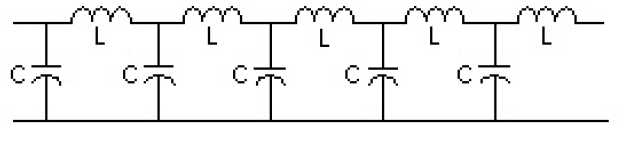
\includegraphics[height=3cm]{tline}
 \end{figure}

 \noindent  We  write the  following  equations  from their  classical
 analogues

 \begin{equation}
   \left\lbrace \begin{aligned}
       V & = -\frac{d\Phi}{dt} = -L\frac{dI}{dt}\\
       I & = -\frac{dQ}{dt} = -C\frac{dV}{dt}
     \end{aligned}\right.\Rightarrow \text{ per unt length}
   \Rightarrow
   \left\lbrace \begin{aligned}
       \frac{dV}{dx} & = - l\frac{dI}{dt}\\
       \frac{dI}{dx} & - c\frac{dV}{dt},
     \end{aligned}\right.
   \label{tlineDiff}
 \end{equation}

 \begin{itemize}
 \item     We    substitute     Eq.\eqref{tlineCurrentVoltage}    into
   Eq.\eqref{tlineDiff} to get

  \begin{equation}
    \left\lbrace \begin{aligned}
        ikV_0&=i\omega lI_0\\
        -i\omega I_0 & = -ickV_0
      \end{aligned}\right. \Rightarrow\left\lbrace \begin{aligned}
        Z_0&=\frac{V_0}{I_0} = \frac{\omega l }{k}\\
        Z_0&=\frac{V_0}{I_0} = \frac{k}{\omega c}\\
      \end{aligned}\right.  \Rightarrow \red{\mathbf{Z_0 =
        \sqrt{\frac{l}{c}}}}\approx
    100\Omega
  \end{equation}

\item We differentiate Eq.\eqref{tlineDiff}

  \begin{equation}
    \frac{d^2V}{dx^2} = -l\frac{d^2I}{dt\partial x} = -l\bigg(-c\frac{d^2V}{dt^2}\bigg) \Rightarrow V_{xx} = \frac{1}{1/lc}V_{tt},
  \end{equation}

  \noindent  which  has the  exact  same  form  as the  wave  equation
  $ y_{xx}=\frac{1}{v^2}y_{tt} $, from which  one can get the speed of
  wave propagation

  \begin{equation}
    \red{v=\frac{1}{\sqrt{lc}}}
  \end{equation}
\end{itemize}

\begin{figure}[h]
  \centering%
  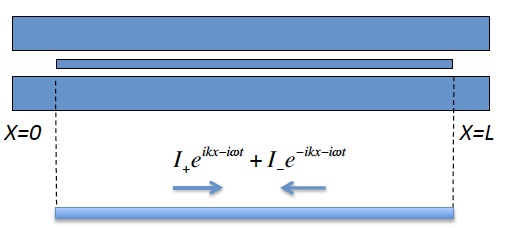
\includegraphics[height=4cm]{res1}%
  \caption{\label{tlineres1}}
\end{figure}

So   far  we   have  had   a  transmission   line  with   no  boundary
conditions. But  now lets us look  at a resonator, depicted  in figure
which has two ends which are cut off and at which

\begin{itemize}
\item \textbf{The current $ I=0 $}: no charge may flow at these points
  of cut.
\end{itemize}

Mathematically speaking

 \begin{equation}
   \left\lbrace \begin{aligned}
       I(x=0) & = I_{+}(x=0)+I_-(x=0)=0\\
       I(x=L) & = I_{+}(x=L)+I_-(x=L)=0
     \end{aligned}\Rightarrow\begin{aligned}
       \red{I_+}&\red{=-I_-}\\
       I_+&= -I_-e^{-i2kL}
     \end{aligned} \Rightarrow \red{k=\frac{\pi n}{L}}, \right.
 \end{equation}

 \noindent and the total current at any point in the resonator will be
 a point on a standing wave

 \begin{equation}
   I(x,t) = I_+(x,t) + I_-(x,t) = I_+e^{i\frac{\pi n}{L}x-i\omega t} - I_+e^{-i\frac{\pi n}{L}x-i\omega t} = {{I_0\sin\bigg[\frac{\pi n}{L}x\bigg]e^{-i\omega t}}}.
   \label{tlineCurrent}
 \end{equation}

 \noindent  Evaluating  the  voltage  using  Eq.\eqref{tlineDiff}  and
 Eq.\eqref{tlineCurrent}

 \begin{equation}
   \begin{aligned}
     \frac{dI}{dx} &= - c\frac{dV}{dt}\\
     kI_0\cos(kx)e^{-i\omega t}& =-c\frac{dV}{dt}\\
     \frac{-1}{i\omega}kI_0\cos(kx)e^{-i\omega t}& =-cV\\
     & \Rightarrow\qquad V &=  -i\frac{k}{\omega c}I_0\cos(kx)e^{-i\omega t}\\
     &&=|Z|I_0\cos(kx)e^{-i\omega t}e^{-i\pi/2}\\
     &&=V_0\cos \bigg(\frac{\pi n}{L}x\bigg)\exp\bigg[-i\omega t-i\pi/2\bigg]\\
   \end{aligned}
 \end{equation}

 \noindent or fully the result is (and depicted in Fig.\ref{tlineVI})

 \red{ \begin{equation}
     \begin{aligned}
       V & =V_0\cos \bigg(\frac{\pi n}{L}x\bigg)\exp\bigg[-i\omega t-i\frac{\pi}{2}\bigg]\\
       I & =I_0\sin \bigg(\frac{\pi n}{L}x\bigg)\exp\bigg[-i\omega t\bigg]\\
       V_0&=|Z|I_0
     \end{aligned}
   \end{equation}}

 \begin{figure}
   \centering%
   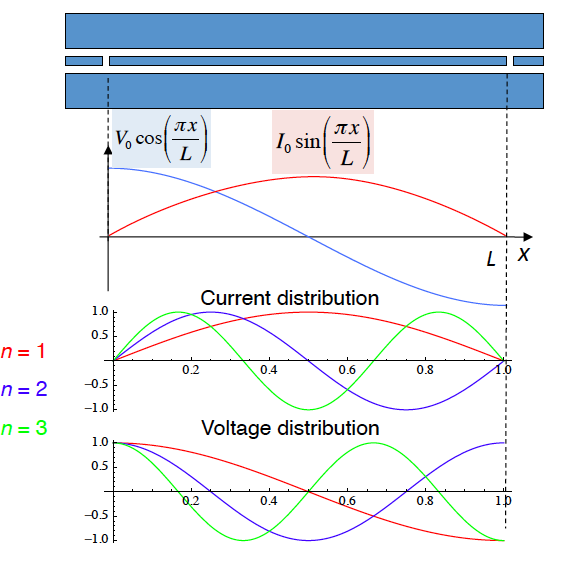
\includegraphics[height=7cm]{vires}
   \caption{Voltage has an  anti-node at the two  sides, while current
     has  a   node.   Multiple  modes   can  be  accomodated   by  the
     resonator\label{tlineVI}}
 \end{figure}

 \subsection{The voltages at the gaps of the resonator}
 Now when  we consider  a boundary,  we shall  label \red{+  as moving
   towards} a boundary, and \blue{- as moving away}.

  \begin{figure}[h]
    \centering%
    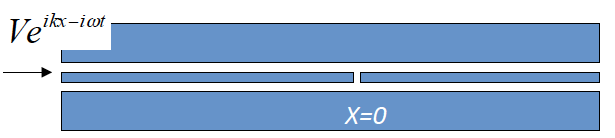
\includegraphics[height=3cm]{gap}
  \end{figure}

  \noindent By defining the transmission and reflection as

 \begin{equation}
   t=\frac{|\blue{V_{R}^{-}}|}{|\red{V_{L}^{+}}|}; \quad r=\frac{|\blue{V_{L}^{-}}|}{|\red{V_{L}^{+}}|}; \quad t=1+r,
 \end{equation}

 \noindent we shall write the propagating waves as follows

 \begin{align}
   \red{V_L^{+}} & = \red{V_0e^{ikx-i\omega t}} \\
   \blue{V_L^{-}} & = \blue{rV_0e^{-ikx-i\omega t}}\\
   \red{V_R^{+}} & = \red{tV_0e^{ikx-i\omega t}},
 \end{align}

 \noindent where  we assume that  no wave  is incident from  the right
 hand  side  ($  V_R^{+}=0 $).   Recalling  Eq.\eqref{tlineDiff}  that
 relates the  current to the  voltage in a  line, let us  evaluate the
 current corresponding to each voltage component in the table below

 \setlength{\extrarowheight}{3mm}
 \begin{table}[h]
   \caption{In               the               last               step
     $     \mathbf{I_0}=V_0\frac{k}{\omega     l}=V_0\frac{1}{v    l}     =
     V_0\frac{\sqrt{lc}}{l} = V_0\sqrt{\frac{c}{l}}=V_0/Z_0 $.}
   \hspace*{-2.5cm}
   \begin{tabular}{|c|c|c|c|c|c|c|c|}
     \hline \textbf{Component} & {Voltage}, $ V $ & \multirow{4}{1.5ex}{$ \Rightarrow $}& $ \frac{dV}{dx} \equiv -l\frac{dI}{dt}$ &\multirow{4}{1.5ex}{$ \Rightarrow $}&  $ \frac{dI}{dt} $ &\multirow{4}{1.5ex}{$ \Rightarrow $}&  Current $ I $ \\\cline{1-2}\cline{4-4}\cline{6-6}\cline{8-8}
     $ \text{Left}\ + $ & $ \mathbf{V_0e^{ikx-i\omega t}} $ & & $ ikV_0e^{ikx-i\omega t} $ && $ -\frac{ik}{l}V_0e^{ikx-i\omega t} $ && $ \frac{k}{\omega l}V_0e^{ikx-i\omega t}  = \mathbf{I_0e^{ikx-i\omega t}}$\\\cline{1-2}\cline{4-4}\cline{6-6}\cline{8-8}
     $ \text{Left}\ - $ & $ \mathbf{rV_0e^{\red{-}ikx-i\omega t}} $ & & $ -ikrV_0e^{\red{-}ikx-i\omega t} $ && $ \frac{ik}{l}rV_0e^{\red{-}ikx-i\omega t} $ && $ -\frac{k}{\omega l}rV_0e^{\red{-}ikx-i\omega t}  = \mathbf{-rI_0e^{\red{-}ikx-i\omega t}}$\\\cline{1-2}\cline{4-4}\cline{6-6}\cline{8-8}
     $ \text{Right}\ + $ & $\mathbf{ tV_0e^{ikx-i\omega t}} $ & & $ iktV_0e^{ikx-i\omega t} $ && $ \frac{ik}{l}tV_0e^{ikx-i\omega t} $ && $ \frac{k}{\omega l}tV_0e^{ikx-i\omega t}  = \mathbf{tI_0e^{ikx-i\omega t}}$\\\hline
   \end{tabular}
 \end{table}

 \begin{framed}\noindent
   Now, the equality of the currents  and voltages on the two sides of
   the  gap  at  $  x=0 $  \red{\textbf{and  including  the  potential
       difference         drop         across         the         gap,
       $      V_{\text{drop}}     =      I_{R}^{+}Z_{\text{gap}}     =
       \frac{tI_0e^{-i\omega   t}}{i\omega  C_{\text{gap}}}   $,  that
       causes the current on the other side of the gap}}

 \begin{equation}
   \left\lbrace\begin{aligned}
       I_0 e^{-i\omega t}-rI_0e^{-i\omega t} & = tI_0e^{-i\omega t}\\
       V_0 e^{-i\omega t}+rV_0e^{-i\omega t} & = tV_0e^{-i\omega t}+\frac{tI_0}{i\omega C_\text{gap}}\\
     \end{aligned}\right.\Rightarrow
   \left\lbrace\begin{aligned}
       1-r & =t\\
       1+r & = \bigg(1+\frac{1}{i\omega C_{\text{gap}}Z}\bigg)t
     \end{aligned}\right.
 \end{equation}
\end{framed}

\noindent and one can simply solve for $ r $ and $ t $ coefficients

 \begin{equation}\label{tLinert}
   \mathbf{\red{t= \frac{1}{1+\frac{1}{i2\omega C_\text{gap}Z}} = \frac{i\alpha}{1+i\alpha};\quad	 r = \frac{1}{1+i\alpha};\quad \alpha = 2\omega C_\text{gap}Z.}}
 \end{equation}

 Now suppose that we defined another gap further down the line. Let us
 see what the resulting voltage at $  x=L $ would be. The voltage that
 is transmitted across the gap initially is $ tV_0 $.

 \begin{figure}[h]
   \centering%
   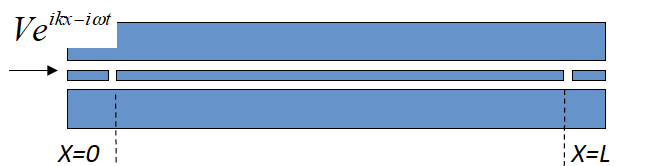
\includegraphics[height=3cm]{gap1}
 \end{figure}

 \begin{multline}\label{tlineMUltiple}
   tV_0 \rightarrow \left\lbrace \text{travels $ L $ to
       $    x=L    $}\right\rbrace    \rightarrow   tV_0e^{ikL-i\omega    t}    \\
   \rightarrow\left\lbrace \text{reflects, travels  $ L $ to  $ x=0 $,
       reflects,  travels  L  to  $  x=L  $  }\right\rbrace\rightarrow
   r^2tV_0e^{ik3L-i\omega t}\\ \rightarrow\left\lbrace \text{reflects,
       travels $ L $ to $ x=0 $, reflects, travels L to $ x=L $
     }\right\rbrace\rightarrow     r^4tV_0e^{ik5L-i\omega      t}     \\
   \rightarrow\left\lbrace \text{reflects, travels  $ L $ to  $ x=0 $,
       reflects,  travels  L  to  $  x=L  $  }\right\rbrace\rightarrow
   r^6tV_0e^{ik7L-i\omega t} \\ \rightarrow\cdots
 \end{multline}

 \noindent so that the total voltage

 \begin{equation}\label{tlineTotalVoltage}
   \begin{aligned}
     V(x=L) & = tV_0e^{ikL-i\omega t}\bigg(1+r^2e^{i2kL}+r^4e^{i4kL}+r^6e^{i6kL}+\cdots\bigg)\\
     & = tV_0e^{ikL-i\omega t}\sum_{n=0}^{\infty}\bigg(r^2e^{2ikL}\bigg)^n, \quad\text{and since $ r<1 $ this is a convergent power series}\\
     & = \mathbf{\frac{tV_0e^{ikL-i\omega t}}{1-r^2e^{2ikL}}.}
   \end{aligned}
 \end{equation}

 \noindent To make good use of this, we need to use

 \begin{equation}\label{tlineApprox}
   \left\lbrace
     \begin{aligned}
       e^{i\alpha+i\alpha^2/2} & = 1+i\alpha +O(\alpha^3) \text{ (proof by simple expansion)}\\
       r & = (1+i\alpha)^{-1} \text{ (from before)}
     \end{aligned}\right.\Rightarrow r^2 \approx e^{-i2\alpha
     +\alpha^2}
 \end{equation}

 \noindent  This  and further  mathematical  stuff  will lead  to  the
 voltage inside the resonator to be

 \begin{equation}\label{tlineVoltage}
   V_r = \frac{V_0}{\alpha}\frac{i(-1)^{n}e^{-i\omega t}}{1+i\frac{2\delta\omega}{\Delta\omega}};\quad \Delta\omega = 2\alpha^2f_0;\quad \delta\omega = \text{ offset from $ n^{th} $ resonance}.
 \end{equation}

 \noindent  \red{As  can  be  seen, the  maximum  voltage  inside  the
   resonator is $ 1/\alpha $ times larger than the external field - we
   have boosted the total field  from the combination of reflections.}
 In a similar way the voltage/power leaving the resonator are

 \begin{equation}\label{tlineLeaving}
   V_{out} = tV_r = \frac{V_0}{\alpha}\frac{i(-1)^{n+1}e^{-i\omega t}}{1+i\frac{2\delta\omega}{\Delta\omega}}; \quad P_{out} = \frac{P_0}{1+\left(\frac{2\delta\omega}{\Delta\omega}\right)^2}.
 \end{equation}


 \red{Important is the  quality factor of the resonator.   This is the
   ratio  of the  resonance frequency  to the  width of  the resonance
   peak}

 \red{\begin{equation}\label{key}                  Q                 =
     \frac{\omega_{\text{resonance}}}{\Delta\omega}=\frac{\pi}{\left(2\omega
         ZC_{gap}\right)^2}.
   \end{equation}}

   \begin{figure}[h]
     \centering%
     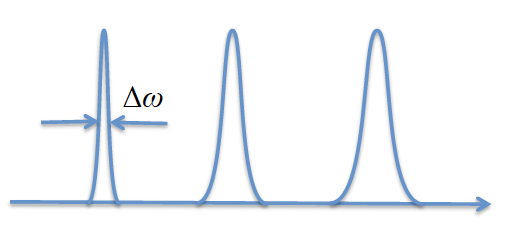
\includegraphics[height=3cm]{res}
   \end{figure}

   Using     results      of     Table.\ref{tab:conversion2},     with
   $      V      =      V_0\bigg(a+a^\dagger\bigg);\quad      I      =
   iI_0\bigg(a-a^\dagger\bigg) $,  and the results from  the classical
   resonator
   $ V=V_0\cos(\frac{\pi n}{L}x);\quad  I=I_0\sin(\frac{\pi n}{L}x) $, the
   quantum field is

   \begin{align}
     \hat{V} & = \sqrt{\frac{\hbar\omega}{2c}}\bigg(a+a^\dagger\bigg)\cos(\frac{\pi n}{L}x)\\
     \hat{I} & = i\sqrt{\frac{\hbar\omega}{2l}}\bigg(a-a^\dagger\bigg)\sin(\frac{\pi n}{L}x)\\
   \end{align}

   \noindent and the total energy, given by the Hamiltonian is

   \begin{equation}\label{tlineTOtalGamil}
     \begin{aligned}
       \mathcal{H} & = \frac{1}{L}\int_{0}^{L}\bigg(\frac{l\hat{I}^2}{2}+\frac{c\hat{V}^2}{2}\bigg)dx \\
       & = \frac{l}{2}\frac{-\hbar\omega}{2l}\bigg(a-a^{\dagger}\bigg)^2\frac{1}{L}\int_{0}^{L}\cos^2(\frac{\pi n}{L}x)dx + \frac{c}{2}\frac{\hbar\omega}{2c}\bigg(a+a^{\dagger}\bigg)^2\frac{1}{L}\int_{0}^{L}\sin^2(\frac{\pi n}{L}x)dx\\
       & = -\frac{\hbar\omega}{4}\frac{1}{2}\bigg(aa-aa^{\dagger}-a^{\dagger}a+a^{\dagger}a^{\dagger}\bigg)+\frac{\hbar\omega}{4}\frac{1}{2}\bigg(aa+aa^{\dagger}+a^{\dagger}a+a^{\dagger}a^{\dagger}\bigg)\\
       &       =       \frac{\hbar\omega}{8}\bigg(aa^{\dagger}+a^{\dagger}a\bigg)=
       \frac{\hbar\omega}{8}\bigg((a^{\dagger}a+1)+a^{\dagger}a\bigg)=\mathbf{\hbar\omega\bigg(\hat{N}+\frac{1}{2}\bigg)},
     \end{aligned}
   \end{equation}

   \noindent so the resonator is a quantum harmonic oscillator.

   \subsection{Resonator types}
   \label{sec:resonator-types}

   \begin{itemize}
   \item  $\lambda/2$   resonator  -  transmission  lines   at  either
     end. Transmission is maximum;
   \item $\lambda/4$ resonator - one end is grounded, other is coupled
     to transmission line. Transmission has a dip.
   \end{itemize}

   \subsection{Resonator Emission}
   \label{sec:resonator-emission}

   This is based off a  slightly related paper \cite{Galli_2009} which
   talks about shining a light on  a cavity. In general, the intensity
   of a signal from a resonator can be fitted by:

   \begin{framed}\noindent
     \begin{equation}
       \text{Intensity} = I_0 + I_1 \frac{\left[ q + 2(\omega - \omega_{0})/\Gamma \right]^2}{1 + \left[ 2(\omega - \omega_0)/\Gamma \right]^2}
     \end{equation}

     \noindent where  apart from scaling  and offset $I_0,  I_1$ there
     is:
     \begin{itemize}
     \item
       $q          =          \frac{\text{Resonant          scattering
           amplitude}}{\text{Non-resonant amplitude}}$;
     \item $\Gamma$ is the FWHM of the scattering (linewidth)
     \end{itemize}
   \end{framed}

   \noindent Light shone on the cavity in \autoref{fig:gali_2009} will
   be reflected in one of two regimes
   \begin{itemize}
   \item Emission at  the cavity frequency and  inevitable emission to
     continuum    (non-resonant)    frequency    \hfill    $q\approx1$
     \autoref{fig:gali_2009}a - asymmetric fit;
   \item Non-resonant emission at a continuum of available frequencies
     \hfill $q << 0$ \autoref{fig:gali_2009}b - flipped lorentzian;
   \item  (Not observed  - very  strong resonant  emission -  standard
     lorentzian) \hfill $q >> 1$.
   \end{itemize}

     \begin{figure}[h]
       \centering \includegraphics[height=6cm]{gali_2009}
       \caption{\small Bigger  area of reflect light  means that there
         is   more    contribution   from    non-resonant   processes.
         \textbf{Note that in  figure B, the lorenztian  is flipped by
           the   experiment  (from   formula  is   should  be   upside
           down).}\label{fig:gali_2009}}
     \end{figure}

\begin{figure}[h]
  \centering 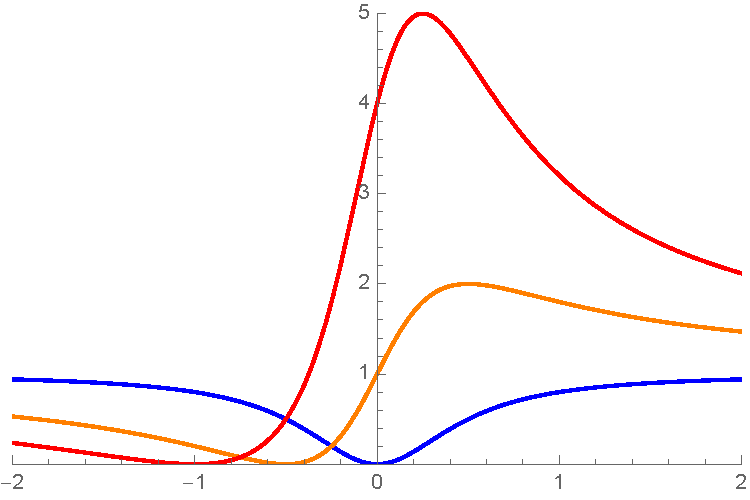
\includegraphics[height=5cm]{mathematica/fano_simulation}
  \caption{\small   Red:   $q=2$,    Orange:   $q=1$,   Blue:   $q=0$.
    \textbf{Note that  when there is  very weak resonant  emission, we
      are centred on the dip,  \red{otherwise the dip will actually be
        off-center}}.\label{fig:fano_simulation}}
\end{figure}

\subsection{Resonator example \cite{Astafiev_2012}}
\label{sec:using-resonators}

In  this  experiment a  $\lambda/2$  resonator  was used  (coupled  to
tranmission line at both ends) which had

\begin{equation}
  \left\{
    \begin{aligned}
      l_{1} & = \frac{L_{sq}}{W} = \frac{0.7\,\text{nH}}{3\,\mum} = 2.3\times 10^{-4}\,\text{H/m} \\
      c_{1} & = 0.85\times 10^{-10}\,\text{F/m}
    \end{aligned}
  \right. \Rightarrow \red{Z_1 = \sqrt{\frac{l_{1}}{c_{1}}} = 1.6\,\text{k}\Omega}, \blue{v = \frac{1}{\sqrt{l_1c_1}} = 7.2\times 10^{6}\,\text{m/s}}
\end{equation}

\begin{framed}\noindent
  \begin{itemize}
  \item Due to the big different  inductance, there would be a current
    maximum at the edges
  \item Only  odd modes will  be coupled, so  that the current  in the
    center of the resonator (where the cqps is) is not zero.
  \item The decay in such a resonator is:
    \begin{equation}
      \kappa = \frac{4Z_{0}}{Z_{1}}\frac{v}{L}.
    \end{equation}

    \noindent
  \end{itemize}
\end{framed}

\begin{figure}[h]
  \centering \inkfig{5cm}{resonator_current_maximum}
  \caption{\small  Maximum current  at  the  interface -  \textbf{very
      different to  the usual case  where there  is no current  at the
      boundaries!}\label{fig:resonator_current_maximum}}
\end{figure}

\subsection{Resonator Fabrication}
\label{sec:reson-fabr}

\begin{framed}\noindent
  Example sizes: \cite{Peltonen_2018}:
  \begin{itemize}
  \item Separation of 20\,\mum from ground plane;
  \item Width of line is 5\,\mum
  \end{itemize}
\end{framed}


To realise,  we put  the atom at  the maximum voltage  of a  `cut out'
resonator.  Full details are given in \cite{Blais_2004}.

\begin{figure}[h]
  \centering 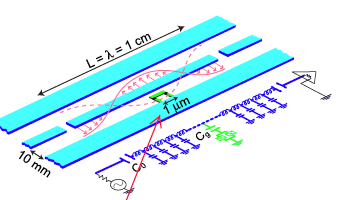
\includegraphics[height=4cm]{cavity_qed_1}
  \caption{Qubit  is  placed  at   the  antinode  of  resonaotr.   The
    tranmission line  itself is modelled  as a sequence  of capacitors
    and inductors.}
\end{figure}

\noindent
\begin{itemize}
\item The coupling  strength is very large because of  the small sizes
  of the elements.  The voltage  between theground plane and resonator
  is 0.2\,V/m,which is 100 times stronger than for a regular cavity;
\item The  geometry of the resonator  fixes its frequency \ira  no 1/f
  noise;
\item Atom  will emit directly into  the line, and with  a high enough
  quality factor, losses are minimised.
\end{itemize}
